
\subsection{Test with $M=N$ on EEG Data Set}

\begin{figure}[H]
    \centering
	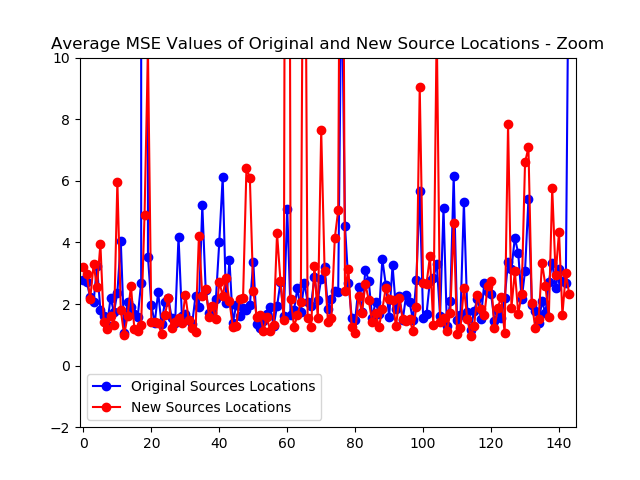
\includegraphics[scale=0.5]{figures/ch_7/M=N_1.png}
	\caption{MSE for system with M=N}
	\label{fig:M=N_1}
\end{figure}  
\begin{itemize}
\item plot \ref{fig:M=N_1} is the case of $N=M$, is to be use as a reference, as that is the 'best' we can archieve. 
\item plot \ref{fig:M=N_test} show that our algorithm can manage to find the almost exact solution in this 'easy' case $N=M$ 
\end{itemize}
\begin{figure}[H]
    \centering
	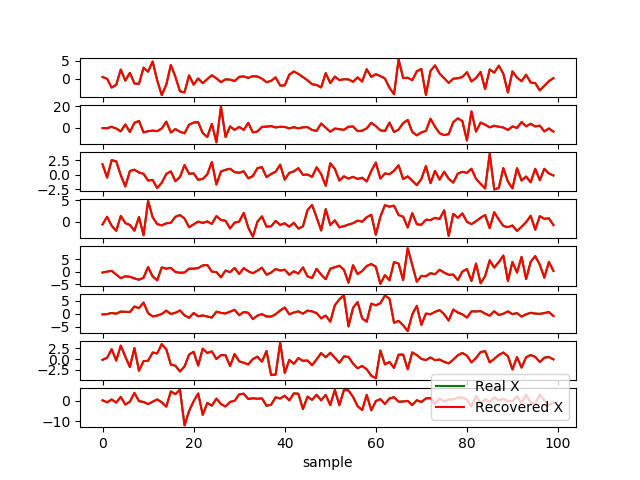
\includegraphics[scale=0.5]{figures/ch_7/M=N_test.png}
	\caption{example to varify tht our system gets the exact result for M=N, MSE is 3.78e-28 }
	\label{fig:M=N_test}
\end{figure}





\subsection{Test with $\frac{1}{3} M<N$ on EEG Data Set}
\begin{figure}[H]
    \centering
	\includegraphics[scale=0.5]{figures/ch_7/M<N_1.png}
	\caption{MSE for system with $\frac{1}{3} M<N$}
	\label{fig:M<N_1}
\end{figure}  
\begin{itemize}
\item  here we have removed $\frac{1}{3}$ of the sensors. The aim is to see if we still can recover the same sources. 
\item plot \ref{fig:M<N_1} is the MSE for every segment, this is to be compared the first plot. It is seen that ...
\item plot \ref{fig:M<N_2} show an example of the recovered sources for one segment, maybe one af few sources should be plotted for better visualisation
\end{itemize}
\begin{figure}[H]
    \centering
	\includegraphics[scale=0.5]{figures/ch_7/M<N_2.png}
	\caption{example of one segment of the system with $\frac{1}{3} M<N$}
	\label{fig:M<N_2}
\end{figure}  






\subsection{Test with $\frac{1}{2} M<N$ on EEG Data Set}
\begin{figure}[H]
    \centering
	\includegraphics[scale=0.5]{figures/ch_7/M<<N_1.png}
	\caption{MSE for system with $\frac{1}{2} M<N$}
	\label{fig:M<<N_1}
\end{figure}  
\begin{itemize}
\item Here we have removed $\frac{1}{2}$ of the sensors. 
\item Plot \ref{fig:M<<N_1} is the MSE for every segment, this is to be compared the first plot. It is seen that ...
\item plot \ref{fig:M<<N_2} show an example of the recovered sources for one segment
\end{itemize}
\begin{figure}[H]
    \centering
	\includegraphics[scale=0.5]{figures/ch_7/M<<N_2.png}
	\caption{example of one segment of the system with $\frac{1}{3} M<N$}
	\label{fig:M<<N_2}
\end{figure} 